% Options for packages loaded elsewhere
\PassOptionsToPackage{unicode,backref,colorlinks=true}{hyperref}
\PassOptionsToPackage{hyphens}{url}
%
\documentclass[
  10pt,
  a4paper,
]{article}
\usepackage{amsmath,amssymb}
\usepackage[]{tgpagella}
\usepackage{ifxetex,ifluatex}
\ifnum 0\ifxetex 1\fi\ifluatex 1\fi=0 % if pdftex
  \usepackage[T1]{fontenc}
  \usepackage[utf8]{inputenc}
  \usepackage{textcomp} % provide euro and other symbols
\else % if luatex or xetex
  \usepackage{unicode-math}
  \defaultfontfeatures{Scale=MatchLowercase}
  \defaultfontfeatures[\rmfamily]{Ligatures=TeX,Scale=1}
\fi
% Use upquote if available, for straight quotes in verbatim environments
\IfFileExists{upquote.sty}{\usepackage{upquote}}{}
\IfFileExists{microtype.sty}{% use microtype if available
  \usepackage[]{microtype}
  \UseMicrotypeSet[protrusion]{basicmath} % disable protrusion for tt fonts
}{}
\makeatletter
\@ifundefined{KOMAClassName}{% if non-KOMA class
  \IfFileExists{parskip.sty}{%
    \usepackage{parskip}
  }{% else
    \setlength{\parindent}{0pt}
    \setlength{\parskip}{6pt plus 2pt minus 1pt}}
}{% if KOMA class
  \KOMAoptions{parskip=half}}
\makeatother
\usepackage{xcolor}
\IfFileExists{xurl.sty}{\usepackage{xurl}}{} % add URL line breaks if available
\IfFileExists{bookmark.sty}{\usepackage{bookmark}}{\usepackage{hyperref}}
\hypersetup{
  pdftitle={tikzplot tests},
  pdfauthor={Andrew Manderson},
  hidelinks,
  pdfcreator={LaTeX via pandoc}}
\urlstyle{same} % disable monospaced font for URLs
\usepackage[margin=2.25cm]{geometry}
\usepackage{graphicx}
\makeatletter
\def\maxwidth{\ifdim\Gin@nat@width>\linewidth\linewidth\else\Gin@nat@width\fi}
\def\maxheight{\ifdim\Gin@nat@height>\textheight\textheight\else\Gin@nat@height\fi}
\makeatother
% Scale images if necessary, so that they will not overflow the page
% margins by default, and it is still possible to overwrite the defaults
% using explicit options in \includegraphics[width, height, ...]{}
\setkeys{Gin}{width=\maxwidth,height=\maxheight,keepaspectratio}
% Set default figure placement to htbp
\makeatletter
\def\fps@figure{htbp}
\makeatother
\setlength{\emergencystretch}{3em} % prevent overfull lines
\providecommand{\tightlist}{%
  \setlength{\itemsep}{0pt}\setlength{\parskip}{0pt}}
\setcounter{secnumdepth}{5}
\usepackage{amsmath}
% I always seem to need tikz for something
\usepackage{tikz}
\usetikzlibrary{positioning, shapes, intersections, through, backgrounds, fit, decorations.pathmorphing, angles, quotes}
\usepackage{lineno}
% \linenumbers


\makeatletter
\@ifclassloaded{imsart}{}{
\usepackage{setspace}
\onehalfspacing
}
\makeatother

\usepackage{relsize}
\usepackage{placeins}

% required for landscape pages. beware, they back the build very slow.
\usepackage{pdflscape}

% table - `gt' package uses these, often unimportant
\usepackage{longtable}
\usepackage{booktabs}
\usepackage{caption}

\usepackage{color}
\definecolor{myredhighlight}{RGB}{180, 15, 32}
\definecolor{mydarkblue}{RGB}{0, 33, 79}
\definecolor{mymidblue}{RGB}{44, 127, 184}
\definecolor{mylightblue}{RGB}{166, 233, 255}
\definecolor{mygrey}{RGB}{68, 68, 68}

\usepackage{colortbl}

\newcommand{\semitransp}[2][35]{\color{fg!#1}#2}

\setcounter{secnumdepth}{3}

\let\Oldcap\cap
\renewcommand{\cap}{\mathrel{\mathsmaller{\Oldcap}}}

% pd stands for: probability distribution and is useful to distringuish
% marignals for probabilities specifically p(p_{1}) and the like.
\newcommand{\pd}{\text{p}}
\newcommand{\q}{\text{q}}
\newcommand{\w}{\text{w}}
\newcommand{\pdr}{\text{r}}
\newcommand{\pdrh}{\hat{\text{r}}}

% melding
\newcommand{\ppoolphi}{\pd_{\text{pool}}(\phi)}
\newcommand{\pmeld}{\pd_{\text{meld}}}

% the q(x)w(x), "weighted target" density 
% for the moment I'm going to call it s(x), as that is the next letter of the 
% alphabet. Can change it later
\newcommand{\s}{\text{s}}
% direct density estimate - replaces lambda.
\newcommand{\ddest}{\text{s}}
% target weighting function
\newcommand{\tarw}{\text{u}}

% constants - usually sizes of things
\newcommand{\Nx}{N}
\newcommand{\Nnu}{\text{N}_{\text{nu}}}
\newcommand{\Nde}{\text{N}_{\text{de}}}
\newcommand{\Nmc}{\text{N}_{\text{mc}}}
\newcommand{\Nw}{W}
\newcommand{\Nm}{M}
\newcommand{\Ns}{S}
\newcommand{\Np}{P}

% locales - could switch to x and x'
\newcommand{\xnu}{x_{\text{nu}}}
\newcommand{\xde}{x_{\text{de}}}
\newcommand{\phinu}{\phi_{\text{nu}}}
\newcommand{\phide}{\phi_{\text{de}}}

% sugiyama stuff
\newcommand{\pdnu}{\pd_{\text{nu}}}
\newcommand{\pdde}{\pd_{\text{de}}}

% indices 
\newcommand{\wfindex}{w}
\newcommand{\sampleindex}{n}
\newcommand{\modelindex}{m}
\newcommand{\stageindex}{s}
\newcommand{\phiindex}{p}

% independence symbol
\newcommand{\indep}{\perp\!\!\!\perp}
\newcommand{\setcomp}{\mathsf{c}}

\newtheorem{theorem}{Theorem}[section]
\newtheorem{corollary}{Corollary}[theorem]

\DeclareMathOperator*{\argmin}{arg\,min}

% ARDS example in text commands
\newcommand{\paoii}{PaO\textsubscript{2}}
\newcommand{\fioii}{FiO\textsubscript{2}}
\newcommand{\spoii}{SpO\textsubscript{2}}
\newcommand{\pfratio}{\paoii/\fioii}
\newcommand{\sfratio}{\spoii/\fioii}
\ifluatex
  \usepackage{selnolig}  % disable illegal ligatures
\fi

\title{tikzplot tests}
\author{Andrew Manderson}
\date{01 July, 2021}

\begin{document}
\maketitle

\begin{figure}
  \begin{minipage}{.49\textwidth}
    % Created by tikzDevice version 0.12.3.1 on 2021-07-01 15:39:56
% !TEX encoding = UTF-8 Unicode
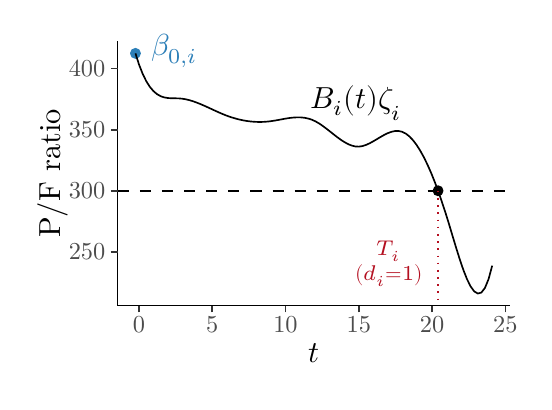
\begin{tikzpicture}[x=1pt,y=1pt,scale=0.9]
\definecolor{fillColor}{RGB}{255,255,255}
\path[use as bounding box,fill=fillColor,fill opacity=0.00] (0,0) rectangle (199.17,142.26);
\begin{scope}
\path[clip] (  0.00,  0.00) rectangle (199.17,142.26);
\definecolor{drawColor}{RGB}{255,255,255}
\definecolor{fillColor}{RGB}{255,255,255}

\path[draw=drawColor,line width= 0.6pt,line join=round,line cap=round,fill=fillColor] (  0.00,  0.00) rectangle (199.17,142.26);
\end{scope}
\begin{scope}
\path[clip] ( 36.11, 30.69) rectangle (193.67,136.76);
\definecolor{fillColor}{RGB}{255,255,255}

\path[fill=fillColor] ( 36.11, 30.69) rectangle (193.67,136.76);
\definecolor{drawColor}{RGB}{0,0,0}
\definecolor{fillColor}{RGB}{0,0,0}

\path[draw=mymidblue,line width= 0.4pt,line join=round,line cap=round,fill=mymidblue] ( 43.27,131.94) circle (  1.96);

\path[draw=drawColor,line width= 0.4pt,line join=round,line cap=round,fill=fillColor] (164.77, 76.78) circle (  1.96);

\path[draw=drawColor,line width= 0.6pt,line join=round] ( 43.27,131.94) --
	( 44.72,127.42) --
	( 46.17,123.73) --
	( 47.61,120.78) --
	( 49.06,118.49) --
	( 50.51,116.78) --
	( 51.95,115.56) --
	( 53.40,114.75) --
	( 54.85,114.26) --
	( 56.29,114.01) --
	( 57.74,113.92) --
	( 59.19,113.90) --
	( 60.63,113.87) --
	( 62.08,113.74) --
	( 63.53,113.49) --
	( 64.98,113.14) --
	( 66.42,112.70) --
	( 67.87,112.18) --
	( 69.32,111.60) --
	( 70.76,110.98) --
	( 72.21,110.33) --
	( 73.66,109.66) --
	( 75.10,108.99) --
	( 76.55,108.33) --
	( 78.00,107.70) --
	( 79.44,107.11) --
	( 80.89,106.58) --
	( 82.34,106.11) --
	( 83.78,105.69) --
	( 85.23,105.32) --
	( 86.68,105.02) --
	( 88.12,104.78) --
	( 89.57,104.59) --
	( 91.02,104.47) --
	( 92.46,104.41) --
	( 93.91,104.41) --
	( 95.36,104.47) --
	( 96.81,104.61) --
	( 98.25,104.80) --
	( 99.70,105.04) --
	(101.15,105.30) --
	(102.59,105.57) --
	(104.04,105.83) --
	(105.49,106.04) --
	(106.93,106.19) --
	(108.38,106.26) --
	(109.83,106.22) --
	(111.27,106.06) --
	(112.72,105.75) --
	(114.17,105.28) --
	(115.61,104.61) --
	(117.06,103.77) --
	(118.51,102.78) --
	(119.95,101.70) --
	(121.40,100.57) --
	(122.85, 99.42) --
	(124.29, 98.30) --
	(125.74, 97.25) --
	(127.19, 96.31) --
	(128.63, 95.52) --
	(130.08, 94.93) --
	(131.53, 94.58) --
	(132.98, 94.50) --
	(134.42, 94.72) --
	(135.87, 95.19) --
	(137.32, 95.85) --
	(138.76, 96.64) --
	(140.21, 97.49) --
	(141.66, 98.36) --
	(143.10, 99.18) --
	(144.55, 99.89) --
	(146.00,100.43) --
	(147.44,100.75) --
	(148.89,100.78) --
	(150.34,100.46) --
	(151.78, 99.75) --
	(153.23, 98.62) --
	(154.68, 97.11) --
	(156.12, 95.21) --
	(157.57, 92.95) --
	(159.02, 90.33) --
	(160.46, 87.39) --
	(161.91, 84.12) --
	(163.36, 80.54) --
	(164.81, 76.67) --
	(166.25, 72.52) --
	(167.70, 68.12) --
	(169.15, 63.46) --
	(170.59, 58.64) --
	(172.04, 53.84) --
	(173.49, 49.22) --
	(174.93, 44.99) --
	(176.38, 41.32) --
	(177.83, 38.39) --
	(179.27, 36.40) --
	(180.72, 35.51) --
	(182.17, 35.91) --
	(183.61, 37.80) --
	(185.06, 41.34) --
	(186.51, 46.72);

\path[draw=drawColor,line width= 0.6pt,dash pattern=on 4pt off 4pt ,line join=round] ( 36.11, 76.78) -- (193.67, 76.78);
\end{scope}
\begin{scope}
\path[clip] (  0.00,  0.00) rectangle (199.17,142.26);
\definecolor{drawColor}{RGB}{0,0,0}

\path[draw=drawColor,line width= 0.6pt,line join=round] ( 36.11, 30.69) --
	( 36.11,136.76);
\end{scope}
\begin{scope}
\path[clip] (  0.00,  0.00) rectangle (199.17,142.26);
\definecolor{drawColor}{gray}{0.30}

\node[text=drawColor,anchor=base east,inner sep=0pt, outer sep=0pt, scale=  0.88] at ( 31.16, 49.24) {250};

\node[text=drawColor,anchor=base east,inner sep=0pt, outer sep=0pt, scale=  0.88] at ( 31.16, 73.75) {300};

\node[text=drawColor,anchor=base east,inner sep=0pt, outer sep=0pt, scale=  0.88] at ( 31.16, 98.26) {350};

\node[text=drawColor,anchor=base east,inner sep=0pt, outer sep=0pt, scale=  0.88] at ( 31.16,122.77) {400};
\end{scope}
\begin{scope}
\path[clip] (  0.00,  0.00) rectangle (199.17,142.26);
\definecolor{drawColor}{gray}{0.20}

\path[draw=drawColor,line width= 0.6pt,line join=round] ( 33.36, 52.27) --
	( 36.11, 52.27);

\path[draw=drawColor,line width= 0.6pt,line join=round] ( 33.36, 76.78) --
	( 36.11, 76.78);

\path[draw=drawColor,line width= 0.6pt,line join=round] ( 33.36,101.29) --
	( 36.11,101.29);

\path[draw=drawColor,line width= 0.6pt,line join=round] ( 33.36,125.80) --
	( 36.11,125.80);
\end{scope}
\begin{scope}
\path[clip] (  0.00,  0.00) rectangle (199.17,142.26);
\definecolor{drawColor}{RGB}{0,0,0}

\path[draw=drawColor,line width= 0.6pt,line join=round] ( 36.11, 30.69) --
	(193.67, 30.69);
\end{scope}
\begin{scope}
\path[clip] (  0.00,  0.00) rectangle (199.17,142.26);
\definecolor{drawColor}{gray}{0.20}

\path[draw=drawColor,line width= 0.6pt,line join=round] ( 44.64, 27.94) --
	( 44.64, 30.69);

\path[draw=drawColor,line width= 0.6pt,line join=round] ( 74.08, 27.94) --
	( 74.08, 30.69);

\path[draw=drawColor,line width= 0.6pt,line join=round] (103.51, 27.94) --
	(103.51, 30.69);

\path[draw=drawColor,line width= 0.6pt,line join=round] (132.94, 27.94) --
	(132.94, 30.69);

\path[draw=drawColor,line width= 0.6pt,line join=round] (162.37, 27.94) --
	(162.37, 30.69);

\path[draw=drawColor,line width= 0.6pt,line join=round] (191.81, 27.94) --
	(191.81, 30.69);
\end{scope}
\begin{scope}
\path[clip] (  0.00,  0.00) rectangle (199.17,142.26);
\definecolor{drawColor}{gray}{0.30}

\node[text=drawColor,anchor=base,inner sep=0pt, outer sep=0pt, scale=  0.88] at ( 44.64, 19.68) {0};

\node[text=drawColor,anchor=base,inner sep=0pt, outer sep=0pt, scale=  0.88] at ( 74.08, 19.68) {5};

\node[text=drawColor,anchor=base,inner sep=0pt, outer sep=0pt, scale=  0.88] at (103.51, 19.68) {10};

\node[text=drawColor,anchor=base,inner sep=0pt, outer sep=0pt, scale=  0.88] at (132.94, 19.68) {15};

\node[text=drawColor,anchor=base,inner sep=0pt, outer sep=0pt, scale=  0.88] at (162.37, 19.68) {20};

\node[text=drawColor,anchor=base,inner sep=0pt, outer sep=0pt, scale=  0.88] at (191.81, 19.68) {25};
\end{scope}
\begin{scope}
\path[clip] (  0.00,  0.00) rectangle (199.17,142.26);
\definecolor{drawColor}{RGB}{0,0,0}

\node[text=drawColor,anchor=base,inner sep=0pt, outer sep=0pt, scale=  1.10] at (114.89,  7.64) {$t$};
\end{scope}
\begin{scope}
\path[clip] (  0.00,  0.00) rectangle (199.17,142.26);
\definecolor{drawColor}{RGB}{0,0,0}

\node[text=drawColor,rotate= 90.00,anchor=base,inner sep=0pt, outer sep=0pt, scale=  1.10] at ( 13.08, 83.72) {P/F ratio};
\end{scope}
\begin{scope}
\definecolor{drawColor}{RGB}{0,0,0}

\node[text=mymidblue,anchor=base,inner sep=0pt, outer sep=0pt, scale=  1.10] at ( 59, 131) {$\beta_{0, i}$};
\node[text=myredhighlight,anchor=base,inner sep=0pt, outer sep=0pt, scale=  1.10] at (145, 45) {$\genfrac{}{}{0pt}{}{T_{i}}{(d_{i} = 1)}$};
\node[text=drawColor,anchor=base,inner sep=0pt, outer sep=0pt, scale=  1.10] at (132,110) {$B_{i}(t)\boldsymbol{\zeta}_{i}$};

\draw[dotted,draw=myredhighlight,line width= 0.6pt] (164.77, 76.78) -- (164.77, 30.69);

\end{scope}
\end{tikzpicture}

  \end{minipage}
  \begin{minipage}{.49\textwidth}
    % Created by tikzDevice version 0.12.3.1 on 2021-07-01 16:42:05
% !TEX encoding = UTF-8 Unicode
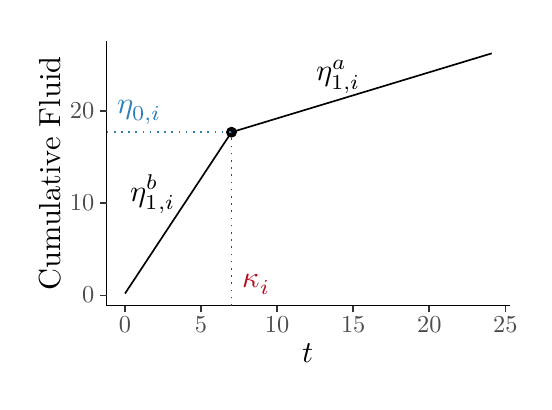
\begin{tikzpicture}[x=1pt,y=1pt,scale=0.9]
\definecolor{fillColor}{RGB}{255,255,255}
\path[use as bounding box,fill=fillColor,fill opacity=0.00] (0,0) rectangle (199.17,142.26);
\begin{scope}
\path[clip] (  0.00,  0.00) rectangle (199.17,142.26);
\definecolor{drawColor}{RGB}{255,255,255}
\definecolor{fillColor}{RGB}{255,255,255}

\path[draw=drawColor,line width= 0.6pt,line join=round,line cap=round,fill=fillColor] (  0.00,  0.00) rectangle (199.17,142.26);
\end{scope}
\begin{scope}
\path[clip] ( 31.71, 30.69) rectangle (193.67,136.76);
\definecolor{fillColor}{RGB}{255,255,255}

\path[fill=fillColor] ( 31.71, 30.69) rectangle (193.67,136.76);
\definecolor{drawColor}{RGB}{0,0,0}

\path[draw=drawColor,line width= 0.6pt,line join=round] ( 39.07, 35.51) --
	( 39.57, 36.25) --
	( 40.06, 37.00) --
	( 40.55, 37.75) --
	( 41.04, 38.49) --
	( 41.54, 39.24) --
	( 42.03, 39.98) --
	( 42.52, 40.73) --
	( 43.01, 41.48) --
	( 43.51, 42.22) --
	( 44.00, 42.97) --
	( 44.49, 43.71) --
	( 44.98, 44.46) --
	( 45.48, 45.20) --
	( 45.97, 45.95) --
	( 46.46, 46.70) --
	( 46.95, 47.44) --
	( 47.45, 48.19) --
	( 47.94, 48.93) --
	( 48.43, 49.68) --
	( 48.92, 50.43) --
	( 49.41, 51.17) --
	( 49.91, 51.92) --
	( 50.40, 52.66) --
	( 50.89, 53.41) --
	( 51.38, 54.16) --
	( 51.88, 54.90) --
	( 52.37, 55.65) --
	( 52.86, 56.39) --
	( 53.35, 57.14) --
	( 53.85, 57.89) --
	( 54.34, 58.63) --
	( 54.83, 59.38) --
	( 55.32, 60.12) --
	( 55.82, 60.87) --
	( 56.31, 61.62) --
	( 56.80, 62.36) --
	( 57.29, 63.11) --
	( 57.79, 63.85) --
	( 58.28, 64.60) --
	( 58.77, 65.35) --
	( 59.26, 66.09) --
	( 59.76, 66.84) --
	( 60.25, 67.58) --
	( 60.74, 68.33) --
	( 61.23, 69.08) --
	( 61.73, 69.82) --
	( 62.22, 70.57) --
	( 62.71, 71.31) --
	( 63.20, 72.06) --
	( 63.69, 72.80) --
	( 64.19, 73.55) --
	( 64.68, 74.30) --
	( 65.17, 75.04) --
	( 65.66, 75.79) --
	( 66.16, 76.53) --
	( 66.65, 77.28) --
	( 67.14, 78.03) --
	( 67.63, 78.77) --
	( 68.13, 79.52) --
	( 68.62, 80.26) --
	( 69.11, 81.01) --
	( 69.60, 81.76) --
	( 70.10, 82.50) --
	( 70.59, 83.25) --
	( 71.08, 83.99) --
	( 71.57, 84.74) --
	( 72.07, 85.49) --
	( 72.56, 86.23) --
	( 73.05, 86.98) --
	( 73.54, 87.72) --
	( 74.04, 88.47) --
	( 74.53, 89.22) --
	( 75.02, 89.96) --
	( 75.51, 90.71) --
	( 76.01, 91.45) --
	( 76.50, 92.20) --
	( 76.99, 92.95) --
	( 77.48, 93.69) --
	( 77.98, 94.44) --
	( 78.47, 95.18) --
	( 78.96, 95.93) --
	( 79.45, 96.68) --
	( 79.94, 97.42) --
	( 80.44, 98.17) --
	( 80.93, 98.91) --
	( 81.42, 99.66) --
	( 81.91,100.31) --
	( 82.41,100.46) --
	( 82.90,100.61) --
	( 83.39,100.76) --
	( 83.88,100.91) --
	( 84.38,101.06) --
	( 84.87,101.21) --
	( 85.36,101.36) --
	( 85.85,101.51) --
	( 86.35,101.66) --
	( 86.84,101.81) --
	( 87.33,101.95) --
	( 87.82,102.10) --
	( 88.32,102.25) --
	( 88.81,102.40) --
	( 89.30,102.55) --
	( 89.79,102.70) --
	( 90.29,102.85) --
	( 90.78,103.00) --
	( 91.27,103.15) --
	( 91.76,103.30) --
	( 92.26,103.45) --
	( 92.75,103.60) --
	( 93.24,103.75) --
	( 93.73,103.89) --
	( 94.22,104.04) --
	( 94.72,104.19) --
	( 95.21,104.34) --
	( 95.70,104.49) --
	( 96.19,104.64) --
	( 96.69,104.79) --
	( 97.18,104.94) --
	( 97.67,105.09) --
	( 98.16,105.24) --
	( 98.66,105.39) --
	( 99.15,105.54) --
	( 99.64,105.68) --
	(100.13,105.83) --
	(100.63,105.98) --
	(101.12,106.13) --
	(101.61,106.28) --
	(102.10,106.43) --
	(102.60,106.58) --
	(103.09,106.73) --
	(103.58,106.88) --
	(104.07,107.03) --
	(104.57,107.18) --
	(105.06,107.33) --
	(105.55,107.47) --
	(106.04,107.62) --
	(106.54,107.77) --
	(107.03,107.92) --
	(107.52,108.07) --
	(108.01,108.22) --
	(108.51,108.37) --
	(109.00,108.52) --
	(109.49,108.67) --
	(109.98,108.82) --
	(110.47,108.97) --
	(110.97,109.12) --
	(111.46,109.27) --
	(111.95,109.41) --
	(112.44,109.56) --
	(112.94,109.71) --
	(113.43,109.86) --
	(113.92,110.01) --
	(114.41,110.16) --
	(114.91,110.31) --
	(115.40,110.46) --
	(115.89,110.61) --
	(116.38,110.76) --
	(116.88,110.91) --
	(117.37,111.06) --
	(117.86,111.20) --
	(118.35,111.35) --
	(118.85,111.50) --
	(119.34,111.65) --
	(119.83,111.80) --
	(120.32,111.95) --
	(120.82,112.10) --
	(121.31,112.25) --
	(121.80,112.40) --
	(122.29,112.55) --
	(122.79,112.70) --
	(123.28,112.85) --
	(123.77,112.99) --
	(124.26,113.14) --
	(124.76,113.29) --
	(125.25,113.44) --
	(125.74,113.59) --
	(126.23,113.74) --
	(126.72,113.89) --
	(127.22,114.04) --
	(127.71,114.19) --
	(128.20,114.34) --
	(128.69,114.49) --
	(129.19,114.64) --
	(129.68,114.79) --
	(130.17,114.93) --
	(130.66,115.08) --
	(131.16,115.23) --
	(131.65,115.38) --
	(132.14,115.53) --
	(132.63,115.68) --
	(133.13,115.83) --
	(133.62,115.98) --
	(134.11,116.13) --
	(134.60,116.28) --
	(135.10,116.43) --
	(135.59,116.58) --
	(136.08,116.72) --
	(136.57,116.87) --
	(137.07,117.02) --
	(137.56,117.17) --
	(138.05,117.32) --
	(138.54,117.47) --
	(139.04,117.62) --
	(139.53,117.77) --
	(140.02,117.92) --
	(140.51,118.07) --
	(141.00,118.22) --
	(141.50,118.37) --
	(141.99,118.51) --
	(142.48,118.66) --
	(142.97,118.81) --
	(143.47,118.96) --
	(143.96,119.11) --
	(144.45,119.26) --
	(144.94,119.41) --
	(145.44,119.56) --
	(145.93,119.71) --
	(146.42,119.86) --
	(146.91,120.01) --
	(147.41,120.16) --
	(147.90,120.31) --
	(148.39,120.45) --
	(148.88,120.60) --
	(149.38,120.75) --
	(149.87,120.90) --
	(150.36,121.05) --
	(150.85,121.20) --
	(151.35,121.35) --
	(151.84,121.50) --
	(152.33,121.65) --
	(152.82,121.80) --
	(153.32,121.95) --
	(153.81,122.10) --
	(154.30,122.24) --
	(154.79,122.39) --
	(155.29,122.54) --
	(155.78,122.69) --
	(156.27,122.84) --
	(156.76,122.99) --
	(157.25,123.14) --
	(157.75,123.29) --
	(158.24,123.44) --
	(158.73,123.59) --
	(159.22,123.74) --
	(159.72,123.89) --
	(160.21,124.04) --
	(160.70,124.18) --
	(161.19,124.33) --
	(161.69,124.48) --
	(162.18,124.63) --
	(162.67,124.78) --
	(163.16,124.93) --
	(163.66,125.08) --
	(164.15,125.23) --
	(164.64,125.38) --
	(165.13,125.53) --
	(165.63,125.68) --
	(166.12,125.83) --
	(166.61,125.97) --
	(167.10,126.12) --
	(167.60,126.27) --
	(168.09,126.42) --
	(168.58,126.57) --
	(169.07,126.72) --
	(169.57,126.87) --
	(170.06,127.02) --
	(170.55,127.17) --
	(171.04,127.32) --
	(171.53,127.47) --
	(172.03,127.62) --
	(172.52,127.76) --
	(173.01,127.91) --
	(173.50,128.06) --
	(174.00,128.21) --
	(174.49,128.36) --
	(174.98,128.51) --
	(175.47,128.66) --
	(175.97,128.81) --
	(176.46,128.96) --
	(176.95,129.11) --
	(177.44,129.26) --
	(177.94,129.41) --
	(178.43,129.56) --
	(178.92,129.70) --
	(179.41,129.85) --
	(179.91,130.00) --
	(180.40,130.15) --
	(180.89,130.30) --
	(181.38,130.45) --
	(181.88,130.60) --
	(182.37,130.75) --
	(182.86,130.90) --
	(183.35,131.05) --
	(183.85,131.20) --
	(184.34,131.35) --
	(184.83,131.49) --
	(185.32,131.64) --
	(185.82,131.79) --
	(186.31,131.94);
\definecolor{fillColor}{RGB}{0,0,0}

\path[draw=drawColor,line width= 0.4pt,line join=round,line cap=round,fill=fillColor] ( 81.84,100.29) circle (  1.96);

\end{scope}
\begin{scope}
\path[clip] (  0.00,  0.00) rectangle (199.17,142.26);
\definecolor{drawColor}{RGB}{0,0,0}

\path[draw=drawColor,line width= 0.6pt,line join=round] ( 31.71, 30.69) --
	( 31.71,136.76);
\end{scope}
\begin{scope}
\path[clip] (  0.00,  0.00) rectangle (199.17,142.26);
\definecolor{drawColor}{gray}{0.30}

\node[text=drawColor,anchor=base east,inner sep=0pt, outer sep=0pt, scale=  0.88] at ( 26.76, 31.74) {0};

\node[text=drawColor,anchor=base east,inner sep=0pt, outer sep=0pt, scale=  0.88] at ( 26.76, 68.76) {10};

\node[text=drawColor,anchor=base east,inner sep=0pt, outer sep=0pt, scale=  0.88] at ( 26.76,105.78) {20};
\end{scope}
\begin{scope}
\path[clip] (  0.00,  0.00) rectangle (199.17,142.26);
\definecolor{drawColor}{gray}{0.20}

\path[draw=drawColor,line width= 0.6pt,line join=round] ( 28.96, 34.77) --
	( 31.71, 34.77);

\path[draw=drawColor,line width= 0.6pt,line join=round] ( 28.96, 71.79) --
	( 31.71, 71.79);

\path[draw=drawColor,line width= 0.6pt,line join=round] ( 28.96,108.81) --
	( 31.71,108.81);
\end{scope}
\begin{scope}
\path[clip] (  0.00,  0.00) rectangle (199.17,142.26);
\definecolor{drawColor}{RGB}{0,0,0}

\path[draw=drawColor,line width= 0.6pt,line join=round] ( 31.71, 30.69) --
	(193.67, 30.69);
\end{scope}
\begin{scope}
\path[clip] (  0.00,  0.00) rectangle (199.17,142.26);
\definecolor{drawColor}{gray}{0.20}

\path[draw=drawColor,line width= 0.6pt,line join=round] ( 39.07, 27.94) --
	( 39.07, 30.69);

\path[draw=drawColor,line width= 0.6pt,line join=round] ( 69.62, 27.94) --
	( 69.62, 30.69);

\path[draw=drawColor,line width= 0.6pt,line join=round] (100.17, 27.94) --
	(100.17, 30.69);

\path[draw=drawColor,line width= 0.6pt,line join=round] (130.71, 27.94) --
	(130.71, 30.69);

\path[draw=drawColor,line width= 0.6pt,line join=round] (161.26, 27.94) --
	(161.26, 30.69);

\path[draw=drawColor,line width= 0.6pt,line join=round] (191.81, 27.94) --
	(191.81, 30.69);
\end{scope}
\begin{scope}
\path[clip] (  0.00,  0.00) rectangle (199.17,142.26);
\definecolor{drawColor}{gray}{0.30}

\node[text=drawColor,anchor=base,inner sep=0pt, outer sep=0pt, scale=  0.88] at ( 39.07, 19.68) {0};

\node[text=drawColor,anchor=base,inner sep=0pt, outer sep=0pt, scale=  0.88] at ( 69.62, 19.68) {5};

\node[text=drawColor,anchor=base,inner sep=0pt, outer sep=0pt, scale=  0.88] at (100.17, 19.68) {10};

\node[text=drawColor,anchor=base,inner sep=0pt, outer sep=0pt, scale=  0.88] at (130.71, 19.68) {15};

\node[text=drawColor,anchor=base,inner sep=0pt, outer sep=0pt, scale=  0.88] at (161.26, 19.68) {20};

\node[text=drawColor,anchor=base,inner sep=0pt, outer sep=0pt, scale=  0.88] at (191.81, 19.68) {25};
\end{scope}
\begin{scope}
\path[clip] (  0.00,  0.00) rectangle (199.17,142.26);
\definecolor{drawColor}{RGB}{0,0,0}

\node[text=drawColor,anchor=base,inner sep=0pt, outer sep=0pt, scale=  1.10] at (112.69,  7.64) {$t$};
\end{scope}
\begin{scope}
\path[clip] (  0.00,  0.00) rectangle (199.17,142.26);
\definecolor{drawColor}{RGB}{0,0,0}

\node[text=drawColor,rotate= 90.00,anchor=base,inner sep=0pt, outer sep=0pt, scale=  1.10] at ( 13.08, 83.72) {Cumulative Fluid};

\end{scope}
\begin{scope}
\definecolor{drawColor}{RGB}{0,0,0}

\node[text=drawColor,anchor=base,inner sep=0pt, outer sep=0pt, scale=  1.10] at (50.40, 72.66) {$\eta_{1, i}^{b}$};
\node[text=drawColor,anchor=base,inner sep=0pt, outer sep=0pt, scale=  1.10] at (124.87,120.90) {$\eta_{1, i}^{a}$};

\node[text=mymidblue,anchor=base,inner sep=0pt, outer sep=0pt, scale=  1.10] at (45, 108) {$\eta_{0, i}$};
\node[text=myredhighlight,anchor=base,inner sep=0pt, outer sep=0pt, scale=  1.10] at (92, 38) {$\kappa_{i}$};

\draw[dotted,draw=mymidblue,line width= 0.6pt] (31.71, 100.29) -- (81.84,100.29);
\draw[dotted,draw=myredhighlight,line width= 0.6pt] (81.84, 30.69) -- (81.84,100.29);

\end{scope}
\end{tikzpicture}

  \end{minipage}
  \caption{test caption}
  \label{fig:test_lab}
\end{figure}

\ref{fig:test_lab}

\end{document}
